% Biot-Savart: Beitrag dB eines Leiterelements d\ell' am Aufpunkt r
% Gemeinsamer Stil für alle Abbildungen (TikZ -> SVG, siehe figures/build.mjs).
%
% Farben sind Platzhalter ("Sentinels"): build.mjs ersetzt sie im SVG durch
% CSS-Variablen, damit die Abbildungen im hellen und dunklen Modus passen.
% Andere Farben (auch schwarz/weiß) bricht der Build mit Fehler ab.
%
%   fg    Linien, Beschriftung          -> --dark
%   mu    Hilfslinien, Achsen, Maße      -> --gray
%   acc   das eine Konzept der Abbildung -> --secondary (Lime/Oliv)
%   blue  zweite Größe, negative Ladung  -> --fig-blue
%   warm  dritte Größe, positive Ladung  -> --fig-warm
%   bg    Seitenhintergrund (Aussparen)  -> --light
%
% Kein \clip verwenden: pdftocairo macht daraus Clip-Gruppen, in denen exakt
% waagerechte/senkrechte Linien verschwinden. Berechnete Kurven schneidet
% gen/*.py selbst am Rahmen ab.
\documentclass[tikz,border=3pt]{standalone}
\usepackage{amsmath,amssymb,bm}
% Text serifenlos wie die Seite, Mathe in Computer Modern wie KaTeX
\renewcommand{\familydefault}{\sfdefault}
\usetikzlibrary{arrows.meta,calc,decorations.markings,patterns,3d,positioning,angles,quotes}

\definecolor{fg}{RGB}{1,2,3}
\definecolor{mu}{RGB}{4,5,6}
\definecolor{acc}{RGB}{7,8,9}
\definecolor{blue}{RGB}{10,11,12}
\definecolor{warm}{RGB}{13,14,15}
\definecolor{bg}{RGB}{16,17,18}

% Vektoren wie auf der Website (KaTeX \mathbf)
\newcommand{\vv}[1]{\mathbf{#1}}

\tikzset{
  every picture/.style={fg, line width=0.8pt, line cap=round, line join=round,
    >={Stealth[length=5.5pt,width=4.4pt]}},
  every node/.style={font=\small},
  % Linientypen
  main/.style={line width=0.9pt},
  thin/.style={line width=0.5pt},
  aux/.style={mu, line width=0.5pt, dash pattern=on 2.5pt off 2pt},
  axis/.style={mu, line width=0.6pt, ->},
  vec/.style={line width=1.1pt, ->},
  field/.style={line width=0.7pt, postaction={decorate},
    decoration={markings, mark=at position #1 with {\arrow{Stealth[length=4.5pt,width=3.6pt]}}}},
  field/.default=0.5,
  % Flächen
  soft/.style={fill=#1, fill opacity=0.14},
  soft/.default=acc,
  % Ladungen
  qpos/.style={circle, fill=warm, inner sep=0pt, minimum size=9pt,
    path picture={\draw[bg, line width=0.9pt] ($(path picture bounding box.center)+(-2pt,0)$) -- +(4pt,0)
      ($(path picture bounding box.center)+(0,-2pt)$) -- +(0,4pt);}},
  qneg/.style={circle, fill=blue, inner sep=0pt, minimum size=9pt,
    path picture={\draw[bg, line width=0.9pt] ($(path picture bounding box.center)+(-2pt,0)$) -- +(4pt,0);}},
  dot/.style={circle, fill=fg, inner sep=0pt, minimum size=3pt},
  % Beschriftung mit Aussparung, damit Linien den Text nicht kreuzen
  lbl/.style={fill=bg, inner sep=1.5pt},
  % Icons: kräftigere Linien, keine Schrift
  icon/.style={line width=1.6pt, >={Stealth[length=6pt,width=5pt]}},
}

\begin{document}
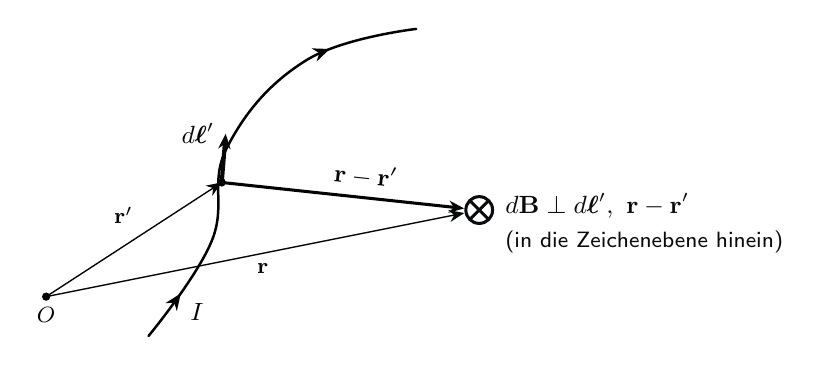
\begin{tikzpicture}
  % Leiter mit Strom I
  \draw[main, postaction={decorate}, decoration={markings,
      mark=at position 0.12 with {\arrow{Stealth[length=6pt,width=5pt]}},
      mark=at position 0.8 with {\arrow{Stealth[length=6pt,width=5pt]}}}]
    plot[smooth, tension=0.7] coordinates {(-0.6,-1.4) (0.2,-0.2) (0.4,1.0) (1.4,2.1) (2.8,2.5)};
  \node[anchor=west] at (-0.2,-1.1) {$I$};
  % Element d\ell' bei r'
  \coordinate (Q) at (0.33,0.55);
  \draw[vec, acc, line width=1.5pt] (Q) -- ++(0.05,0.62) node[anchor=east] {$d\boldsymbol\ell'$};
  % Ursprung, Aufpunkt
  \coordinate (O) at (-1.9,-0.9);
  \coordinate (P) at (3.6,0.2);
  \node[dot] at (O) {}; \node[mu, anchor=north, font=\footnotesize] at (O) {$O$};
  \draw[vec, mu, thin] (O) -- (Q) node[pos=0.55, anchor=south east, text=mu, font=\footnotesize] {$\vv r'$};
  \draw[vec, mu, thin, shorten >=5.5pt] (O) -- (P) node[pos=0.5, anchor=north, text=mu, font=\footnotesize] {$\vv r$};
  \draw[vec, shorten >=5.5pt] (Q) -- (P) node[pos=0.55, anchor=south, sloped] {$\vv r-\vv r'$};
  \node[dot] at (Q) {};
  % dB = dl' x (r-r'): z-Komponente 0.05*(-0.35) - 0.62*3.27 < 0 -> in die Ebene hinein
  \draw[blue, line width=1.1pt] (P) circle (0.17);
  \draw[blue, line width=1.1pt] ($(P)+(-0.11,-0.11)$) -- ++(0.22,0.22) ($(P)+(-0.11,0.11)$) -- ++(0.22,-0.22);
  \node[blue, anchor=west] at ($(P)+(0.2,0.05)$) {$d\vv B\perp d\boldsymbol\ell',\ \vv r-\vv r'$};
  \node[blue, anchor=west, font=\footnotesize] at ($(P)+(0.2,-0.4)$) {(in die Zeichenebene hinein)};
\end{tikzpicture}
\end{document}
